% ch: General concepts about blockchain applications

The blockchain technology has emerged in the context of Bitcoin crypto-currency as a proposal to solve the double-spending problem presented in a transaction of digital money, i.e., the capability to exchange the same amount more than once.
For instance, it is like if someone uses the ``same'' cash in different places because the accuracy of fake money copies don't call attention until its go back to central bank, where identifiers are checked. % o número de registro não é verificado nos bancos comuns?

Independently of the kind of money, the current veracity analysis for any transaction between stakeholders is made by a third-party trustful by them.
Its a common approach which uses an impartial stakeholder capable to certify each transaction, and to store the history of exchanges in a database, also called ledgers.
This method of data management increases transaction costs, that limits minimum practical values and small deals, however, it guarantees the action of reversal transactions when needed~\cite{satoshi2009}.

Thus, the Bitcoin solution was a protocol that uses a \gls{p2p} network architecture
with a controlled redundancy of transactions registrations
in a write-only format
verified by each user in its network in order to allow
``transactions that are computationally impractical to reverse [that] would protect sellers from fraud,
and routine escrow mechanisms [\dots] to protect buyers''~\cite{satoshi2009}.

But the blockchain technology goes beyond money applications, it can be used to track any asset transaction, and it represents a new form of information management that can potentially impact the whole society.
Since the trustful intermediary is indeed the blockchain network, where users agree upon how it operates to reach a consensus about the validity of a transaction~\cite{swan2015blockchain},
several blockchain technologies have arisen to fit all kinds of business~\cite{gartner}.
% gancho para dapps e explicar diferença entre tipos de blockchain e frameworks.

However, due to its initial stage, there are some mismatched terminologies.
For instance, the word \emph{blockchain} has been using to the data structure~\cite{xu2017} reproduced by and stored at nodes, i.e., the ledger registrations.
And the cryptographically decentralized network connecting each node, represented by a \gls{p2p} communication overlay network with a consensus method is referred to \emph{blockchain technology}~\cite{xu2016} or \emph{\gls{dlt}}~\cite{itu2017}.
Therefore, some standards are under development to cope with it and to define the better use and compatibility between companies and services, such as the technical committee \emph{ISO/TC 307 - Blockchain and distributed ledger technologies}
\footnote{\href{https://www.iso.org/committee/6266604.html}{https://www.iso.org/committee/6266604.html}}, and
the IEEE Standards Association (IEEE-SA) through the \emph{IEEE Blockchain Initiative (BCI)}
\footnote{\href{https://blockchain.ieee.org/standards}{https://blockchain.ieee.org/standards}}.
% Falta falar do grupo de discussão ITU-T!
% https://www.itu.int/en/ITU-T/focusgroups/dlt/Pages/default.aspx
% E dos grupos especiais de integração da blockchain com TE!

Briefly, two analogies portray well what the blockchain technology is for the business application point of view.
One can be seen as a big digital ledger shared by all those who participate in the system, in which transactions are irreversibly recorded.
It is the chronological record of all transactions compiled and validated that occurred in the network.
It is unique and shared by a specific system~\cite{block-endeavor}. % Endeavor [2015]
And the other can be said that the blockchain is like a reef of coral in which only the last millimeters represent active biomass, the rest is only a dead image of the past and accessed only on rare occasions to check historical data~\cite{blocktrading}. % Merz [2016]
%Cara, Parabens por esse paragrafo! Cabuloso.

As noted in \nameref{ch:0}, the blockchain technology components are not new if analyzed separately.
Distributed networks, and public and private keys cryptography have been part of our daily life for years,
however the novelty is in how to generate and communicate consensus on a common redundant database updated through a decentralized network~\cite{its2}.
This behaviour and the main blockchain terms are described in \autoref{sec:terms}.
Thereafter, \autoref{sec:timeline} exposes a brief evolution of the blockchain technology.
Following, some relevant blockchains are presented in \autoref{sec:varieties},
as well as some of its astonishing \glspl{dapp} in \autoref{sec:dapp}.

\section{Terminology and characteristics}
\label{sec:terms}

% ... Intro par...
% "Seen as a data structure, the blockchain is an ordered list of blocks.
% Blocks are the containers % isso é um termo técnico
% aggregating transactions.
% Every block is identifiable, and linked back to its previous block in the chain."~\cite{xu2016}

As a \gls{p2p} network, the blockchain technology has some functionalities inherited from the aforementioned architecture, such as
\begin{enumerate*}[label={(\roman*)}]
    \item the peers can leave and join the network anytime~\cite{satoshi2009,book:p2p-mob},
    \item the presence of some ``special'' peers with distinguish characteristic (eg. processing power) in order to ``perform complex functions such as indexing, query processing, access control, and meta-data management''~\cite{book:p2p-mob},
    \item each peer is both a client and a server which are normally convenient for large-scale applications~\cite{book:p2p-mob},
    \item an overlay network
    % \footnote{Precisely, the PetalUp-CDN approach that is used to distribute web content in the Internet, alternatively to the traditional web servers.}
    designed to have scalability with low costs, without compromise peer autonomy~\cite{book:p2p-mob}, and
    \item the growth of the network resource and content availability is proportional to the number of peers, but the network keeps an invariable response time, and a high search throughput~\cite{book:p2p-mob}.
\end{enumerate*}

However, they keep apart on the manner the network is used by its applications.
While traditional \gls{p2p} networks share computer resources (content, memory, storage, processing, bandwidth, and so on) to achieve scalability for content distribution~\cite{book:p2p-mob}, % bittorrent compartilha o quê?
the blockchains achieve the same requirement replicating the data structure across the peers guaranteeing interoperability.
Although good for data retrieving and reliability, it represents a limit on the file data size and on the data structure.%~[ref].

In addition, the participants of this network can be split into two node types:
\begin{enumerate*}[label={(\roman*)}]
    \item one that just uses the network as a service to communicate directly with peers, to contribute to a transaction verification and to store information, and
    \item another (the ``special'' peer) that works to keep the network organized, appending new blocks of information on the ledger.
\end{enumerate*}
The latter is responsible to integrate the consensus method about the new information to be spread and updated across the network.

Every node has two \emph{cryptographic keys} to keep its connections reliable.
While the public key is for information traceability, the private key is used to certify the data ownership in a transaction.

The \emph{transaction} is indeed any message about some arbitrary operation in the network.
For instance, it can be an exchange between peers, an entity registration, or yet the creation of cryptocurrencies.
It is supported by the so-called \emph{smart contracts}, that just minimize the need for a trustful third-party to solve the same common problem~\cite{swan2015blockchain}.
Its arbitrates an agreement between peers, being basically a business logic running on the blockchain~\cite{hyper2}.

However, besides businesses logics written by ordinary programmers, each blockchain technology has its particularity to handle with all sort of contracts.
This establishes two different types of smart contracts.
One of them acts on the network nodes validators. They are pre-build smart contracts with installed features essentials to deal with all the network functionalities.
The other is the on-chain smart contract, which follow business purposes and are deployed as a transaction. When successfully appended on the ledger, their codes are part of the network and available to be called by subsequent transactions~\cite{hyper2}.

The relationship between these two smart-contracts defines the blockchain system behaviour and how an on-chain smart contract are processed in front of possible errors and validations.
Briefly, a on-chain smart contract can be divided into three parts:
\begin{enumerate*}[label={(\roman*)}]
    \item the inputs gather the contract identifier, the transaction request, any dependencies that may exist, and the current state of the ledger;
    \item the interpreter has the information about the ledger current state and the smart contract code itself;
    \item the outputs have the new transaction state (accepted/rejected) and any side effects, as a notification of something
\end{enumerate*}
~\cite{hyper2}.

Therefore, when a smart contract transaction is processed, the inputs are immediately checked by the interpreter in order to reject any invalid request.
The outputs are generated accordingly with the verification, resulting in different values if the request was valid and accepted, or has raised any errors.
From here, the upcoming steps are handled by the installed smart contracts, i.e., this depends on the particular behaviour of each blockchain technology.
They are responsible to define what has to be done with the transaction based on the output.
If the transaction is ready to be appended on the ledger, the consensus service is called,
otherwise the error service is called~\cite{hyper2}.

Independently of the error type, the crucial feature to be considered is how the blockchain deal with the new state produced by a smart contract transaction.
An analysis considered case by case, because the smart contracts may establish a transaction restriction at execution time, differently than conventional applications, with rules settled at the entire database or at application levels.~\cite{itu2017}.
% Talvez o que se queira dizer é sobre a imutabilidade do código, não?
Furthermore, as a code infrastructure governing the exchanges, the smart contracts can be also fully automated to be triggered when specific future event happens in a certain time frame~\cite{swan2015blockchain, xu2017},
taking advantage of lower costs for contracting, enforcement, and compliance~\cite{itu2017}.
% Sao poucas as blockchain que fazem esse trigger on chain ainda (VITOR)
However, the trigger feature is not so simple to implement due to the monitoring condition of the blockchain status may rely on off-chain mechanisms, and because of the personalized structure of each smart contract.

% Acho q vou tirar isso
% Although the blockchain applications can be economically viable for low-value business transactions~\cite{itu2017},
% there are some risks involved, such as the immutability of the smart contract code -- limiting future improvements or bug arrangements~\cite{itu2017}.

To complement a transaction process, nodes must reach \emph{consensus} about the veracity of the information to be appended in the network.
An automated distributed mechanism is used to regulate
\begin{enumerate*}[label={(\roman*)}]
    \item the criteria that the new items should meet to be added,
    \item how the incentive scheme works for the (``special'') peers responsible for that, and
    \item how the possible conflicts are solved
\end{enumerate*}~\cite{xu2017}.
Thus, consensus must satisfy the properties of:
\begin{enumerate*}[label={(\roman*)}]
    \item \textit{safety} because it has to guarantee that each node has the same output for the same sequence of inputs, i.e., keep the system behaviour equal for every node when a change may occur in a given node; and
    \item \textit{liveness} since each non-faulty node must ultimately receive every submitted transaction in the absence of communication troubles
\end{enumerate*}
~\cite{hyper1}.
This is an odd characteristic of blockchain systems, which indeed is used for classifying a range of \gls{dlt}'s.
Therefore, some kinds of consensus algorithm are described below:
\begin{description}[font={\normalfont\bfseries}]
    \item[\glsitem{pow}] is a random process to discover a transaction hash number~\cite{pwc2016, xu2016}.
    It is a hard task to accomplish with, so nodes with high processing capacity has advantages front of others~\cite{xu2016}.
    Additionally, some conditions to satisfy the system latency and speed increase the task difficulty~\cite{pwc2016}.
    It is not for nothing that those ``special'' nodes are called miners~\cite{itu2017}.
    Right after the hash number has been found, the process is validated throughout every node.
    When the majority of nodes has done it, the transaction is confirmed to the counterparties, because most of its outputs have already been appended in the ledger~\cite{pwc2016}.
    \gls{pow} is very costly to produce but easy to be verified, and the transaction processing rate is limited by the network consensus rules~\cite{xu2016}.
    % Detailed description available on the Chapter 8 of \citeonline{book:bitcoin}.
    
    \item[\glsitem{pos}] simplifies the \gls{pow} method by distributing the verification process between peers proportionally to their shares of the network~\cite{pwc2016}.
    So, if a peer has 10\% sharing of the total blockchain assets, it will have to deal with 10\% of the mining process.
    This approach reduces the complexity, the energy use and the operating costs of an entire transaction step~\cite{itu2017}.
    Due to its openness to being part of the block generation network relies on financing sharing, the crypto-currency process uses to be referred to as minted~\cite{itu2017}.
    In addition, at \gls{pos} blockchains, any malicious attack would require a large amount of currency to work out, which is very expensive~\cite{xu2016}.
    
    % \item[\glsitem{pob}] is the protocol used by the Counterparty platform to extend the Bitcoin blockchain basic financial feature towards the development of \glspl{dapp}.
    % Its process involves the creation of its own crypto-currency, called XCP, burning Bitcoins, i.e.,
    % the peers have to send Bitcoins to an unspendable Bitcoin address to get XCP in exchange~\cite{xu2016}.
    % Mas como monitora que foi para o endereço certo?
    % Preciso criar uma conta primeiro na Counterparty para isso funcionar?
    % RELER: https://en.bitcoin.it/wiki/Proof_of_burn --> 04/02/19
    
    % \item[\glsitem{por}] is ....
    % "More recently, Permacoin proposes a modification to Bitcoin [17], which uses “Proof-of-retrievability” to re-purpose Bitcoin’s mining resource to distributed storage of archival data. This approach provides additional incentives to contribute resources to the network."~\cite{xu2016}
    
    \item[\glsitem{poet}] is another alternative to \gls{pow} developed by Intel that is a hybrid of a random lottery%
    \footnote{\href{https://en.wikipedia.org/wiki/Random_number_generation}{\textcolor{red}{Isso?}}}
    and first-come-first-serve basis algorithm~\cite{LFS171x}.
    Basically, the validator peers%
    \footnote{\textcolor{red}{Como são definidos?}}
    receive a random wait time to execute a given request.
    The one with the shortest wait time wins the dispute to create the next block on the chain~\cite{LFS171x, poet}.
    The \gls{poet} uses new secure CPU instructions, as a \gls{tee}%
    \footnote{\href{https://en.wikipedia.org/wiki/Trusted_execution_environment}{It is an isolated secure CPU area with confidential and integrity performance. More information at Wikipedia.}}%
    , to ensure the safety and randomness of the peer election process as an alternative to the costly investment of power and specialized hardware~\cite{poet}.
    
    \item[\glsitem{pbft}] is one of the algorithms used to solve the Byzantine Generals Problem%
    \footnote{\href{https://achainofblocks.com/2018/08/09/byzantine-generals-problem-proof-of-work/}{The Byzantine Generals Problem and Blockchain Consensus Model Proof of Work | A Deep Dive}}
    , i.e., to keep a distributed networking reliable and functional in the presence of failures of any nature (hardware or software).
    Although the Byzantine Fault Tolerance mechanism is a universal solution for system communication interferences,
    and all the aforementioned consensus methods are considered solutions to this problem,
    the following protocols are optimizations of the \gls{pbft} only~\cite{neowp, LFS171x}.
    However, either the \textbf{\glsitem{sbft}}~\cite{LFS171x} and the \textbf{\glsitem{dbft}}~\cite{neowp} have a single validator, known and trusted by all peers in the network, responsible to append new blocks in the ledger.
    And the consensus is a result of the interaction of some other nodes ratifying the truthfulness of the transactions.
    In the end, the process must comply with the consensus of $2f+1$ nodes in a system with a total of $3f+1$ nodes, where $f$ is the number of faults.
    Thus, both keep good performance front of the network scalability.

    \item[\glsitem{poa}] turns the nodes allowed to create new blocks and append them on the ledger identifiable, making their personal information available for cross-reference.
    Based on their responsibility in the network, they are called ``authorities'', and there are no need of mining to reach consensus, because each authority is carefully choose and rewarded to validate the transactions on behalf of the network interests~\cite{LFS171x}.
    At the \gls{poa} the peer reputation is enough to keep the network trustworthy.
\end{description}

% Discussão sobre as diferenças:
Summing up, the different ways to get consensus stand on different network resources and fault tolerance models, which can be through the use of lottery-based algorithms -- \gls{poet} and \gls{pow} --, or through the use of voting-based methods -- \gls{pos}, \gls{poa} and \gls{pbft} optimizations~\cite{hyper1}.
The former kind of algorithms has a good scalability factor~\cite{LFS171x}, although \gls{pow} does not perform well for the speed and finality of the consensus, i.e., a transaction verification last long and a fork on the network may invalid a given transaction.
Otherwise, the latter kind provides low-latency finality%
\footnote{"Latency -- the time it takes from the creation of a transaction until the initial confirmation of it being accepted by the network (and how the confidence of acceptance increases over time)"}%
% https://hackernoon.com/latency-and-finality-in-different-cryptocurrencies-a7182a06d07a
% LOW LATENCY definitions - informatic and economic
% https://www.informatica.com/services-and-training/glossary-of-terms/low-latency-definition.html#fbid=myswTUZ-A8Y
~\cite{LFS171x} but not so good scalability performance, because the trade-off between these both specifications relies on the number of nodes responsible to append data in the network.

Finally, the \gls{ico} is an alternative mechanism to distribute tokens for users of a given blockchain.
Its usually represents a crowdfunding for a \gls{dapp} development,
either because of the way tokens are distributed by fundraising,
or because of the predefined mechanism to generate the tokens~\cite{pwc2016}, usually a different process than the one used to create native crypto-currency.
Moreover, the distinctive token lets the \gls{ico}'s representative weights the coins from another crypto-currency, instead of relying on fiat-money.

\subsection*{Basic Properties}
\label{ssec:properties}

\textcolor{red}{REESCREVER! Tem muita confusão sobre o que é requisito, especificação, o que se refere a protocolo de redes, o que se refere a ``avaliação'' de uma aplicação... É necessário ter isso claro para descrever a \autoref{tab:de-centralisation} e para comparar os tipos de blockchains na próxima seção.}

In general, the design of any computer network must meet technological and social compliance.
The former includes connectivity features (cost-effective, fair and robustness),
and flexibility to integrate with future changes (from underlying technologies to new demands by applications).
The latter refers to accessibility by humans with different levels of skill~\cite{book:net-sys}.

The properties of \gls{p2p} systems have some advantages in relation to client-server ones, such as scalability, % (cost)
autonomy and dynamic behaviour of peers,
self-organization,
decentralization, and
fault-tolerance % (reliability)
~\cite{book:p2p-mob}.
But blockchains add the properties of
immutability, % (write-only)
non-repudiation, % (irreversible)
integrity,
transparency, and
equal rights~\cite{xu2017}.
Although they complement each other, there is a fine line between what stands for blockchain applications and for network infrastructure.

In addition, some of those properties may be adjusted to give rise to different blockchains.
For instance, a different arrangement of data privacy can allow new options to read the ledger.
The scalability factor and latency between submission and confirmation of a transaction can be impacted by the consensus protocol~\cite{xu2017}.
The set combination of these requirements differs extremely across industries and business use cases, which is a unique optimization opportunity for the technology~\cite{hyper1}.
Further analysis about it is presented at \autoref{sec:varieties}.

\section{Timeline}
\label{sec:timeline}

The blockchain technology has been evolving since Bitcoin appearance, which has constituted the first generation of the \gls{dlt}, remarkable by the decentralization of money and payments.
Succeeding, the second generation stands for the decentralization of markets in general, because the transactions can be made with any kind of asset.
At this time, a good understand of smart contract behaviour guides actions towards current models replacement, that supports the development of \emph{\glspl{dapp}}.
Last but not least, it is expected from the third generation a completely autonomy management system with smart contracts,
a perspective capable to revolutionize the market due to its complexity~\cite{swan2015blockchain}.

Nowadays, we are experiencing a variety of \glspl{dapp} ranging from online card games%
\footnote{\textcolor{red}{Não achei exemplos ainda...} \href{Outros casos a se considerar!}{https://medium.com/crowdbotics/examples-of-blockchain-games-and-how-they-work-7fb0a1e76e2e}}
to popular initiative bills support% bill = draft law
\footnote{The application \emph{Mudamos} strengthens the relationship between Brazilian voters and their representatives collecting their electronic signatures to enforce law changes. More information in Portuguese at \href{https://www.mudamos.org/}{https://www.mudamos.org/}.}.
Although it lacks formal definition, in the most cases, the \glspl{dapp} are open source platforms to work at,
dependent of fee to be executed,
and controversial about code adaptability for future adjusting.
However, there are consent that a \gls{dapp} is one or more smart contracts that runs in a decentralized network securely protected with a special feature of distributed storage functionality and data management~\cite{swan2015blockchain, pwc2016}.
In addition, the \glspl{dapp} ecosystem are vast with no clear target market defined by service providers, which results in different applications categories beyond the \gls{dlt} classification development, i.e.,
a given blockchain framework used to breakthrough a food supplychain system can fit as well a grocery store payment system~\cite{gartner}.

\section{Blockchain varieties}
\label{sec:varieties}

The projects with blockchain vary in its value proposition according to the market purpose, i.e.,
if it aims to manage operations between enterprises, or within a single company~\cite{gartner}. % Kandaswamy [2016]
In addition, the degree of integration with a mechanism of payment processing should be considered as well.
If the project is only intended for data communication or for synchronization of participants' applications, there are no special requirements.
However, if the participants' interactions are used for accounting purposes, this can be done defining different levels of data access and share~\cite{blocktrading}.
In other words, the type of blockchains can be categorized as the way its users agree on how to reach consensus~\cite{itu2017}.

Therefore, the blockchain technology has been designating as \emph{permissionless} and as \emph{permissioned}~\cite{itu2017,peck2017}.
Although both are ``similarly designed for rapid detection of unauthorized changes to the data''~\cite{itu2017},
the latter aims to overcome some challenges presented on the former~\cite{peck2017}.
At permissionless blockchains, the consensus process and the access to read the ledger are open to everyone, i.e., the \gls{dlt} has no owner.
That's why it is also referred to as public blockchains, keeping the attributes of decentralization, no censorship, no counterparty exposure, and an open, global membership~\cite{itu2017}.

However, at permissioned blockchains, participants may be preselected, and the process of read and write the ledger may be restricted for different users~\cite{itu2017}.
It is usually split into ``permissioned public'' and ``permissioned private''.
The latter may have one or many owners, and the consensus method is limited by someone.
The former configures as a trade-off in between the latter and the permissionless blockchains.
Even though the latter is more restrictive, it allows a more efficient way to append data and faster verification processes.
Which means a direct correlation among the trust factor, the computational power required for consensus, and the speed of a transaction~\cite{itu2017}.

There is a belief that this categorization may be more granular~\cite{itu2017}.
% ,even so, its range by what is shown in Table \ref{tab:blocks-classif} so far.
For instance, a permissioned private blockchain, also referred to as \gls{baas}, can be easily compared with a secure append-only database
with similar ``functionalities as a standard cloud-hosted application, with suitable access control and identity regime, that records specific actions of those involved in an appropriate `secure' database''~\cite{singh2017}.
However, it lacks the sense of self-organized community in a trustfulness environment~\cite{peck2017},
although being able to develop a new cloud computing marketplace based on the decentralized approach proposed by blockchain systems, such as the case of iExec%
\footnote{\href{https://iex.ec/}{https://iex.ec/}}.

Based on the work from \citeonline{xu2017},
it is possible to understand how the basic specifications of blockchains compose some of the systems available in the market.
The publishings from \citeonline[p.~35]{peck2017} and \citeonline[p.~19]{uk2016} complement the aforementioned view with workflow guides to determine if a given application should be based or not on a blockchain.
\autoref{tab:de-centralisation} shows different informational system designs comparing their weaknesses and strengths.
% MOOC: Blockchain: Understanding Its Uses and Implications : graph to decide the use based on data store and access!
% Quais são as premissas utilizadas em cada fluxograma? Todas estão relacionadas ao compartilhamento/armazenamento de dados?
% Em que se difere de um sistema distribuído? Pq só comparam com um database centralizado?

The fundamental properties are the basic requirements previously cited at \autoref{ssec:properties} -- immutability, non-repudiation, integrity, transparency, and equal rights.
\textcolor{red}{Resumir o que foi detalhado em \autoref{ssec:properties}.}

The cost efficiency, the performance, and the number of failure points are a result from a trade-off analysis made by \citeonline{xu2017} about what data and computation should be placed on- and off-chain.
\textcolor{red}{Descrever como essas variáveis foram medidas e dar exemplos.}

The verifier statement represents the possibilities available to reach consensus about a certain transaction.
\textcolor{red}{Completar com a descrição dos tipos de consensos, que inclusive já estão como exemplos. Falar de forma ``lottery-based''...}

\textcolor{red}{NUMBER OF FAILURE POINTS: qual a diferença de análise entre o primeiro quadro e o segundo?}

Note that the separation between the network classification to the consensus types evidences the potential range of blockchain configurations.
Moreover, permissionless and permissioned blockchains can be identified too.
\textcolor{red}{E que essa classificação não depende do tipo de consenso utilizado.}

\begin{table}[h!tbp]{\textwidth}
    \centering
    \caption{Systems design decisions regarding (de)centralisation, and their relative impact based on basic properties.}
    \label{tab:de-centralisation}
    \frame{\def \cw {p{1cm}} % column width
\tiny
% \scriptsize
% \footnotesize
% \small
\begin{tabular}{m{2.5cm} m{5.5cm} m{1.3cm} m{1.3cm} m{1.3cm} m{1.3cm}}
    
     & & \multicolumn{4}{c}{\textbf{Impact}}\\\cline{3-6}
    
    \multirow{-2}{*}{\textbf{Decision Design}} & \multirow{-2}{*}{\textbf{Option}} & \textbf{Fundamental properties} & \textbf{Cost efficiency} & \textbf{Performance} & \textbf{\# Failure points}\\\hline
    
    \multirow{3}{*}{Fully Centralised} & \multicolumn{1}{m{5.5cm}|}{Services with a single provider (e.g. governments, courts)} & \multicolumn{1}{c|}{\multirow{3}{*}{$\oplus$}} & \multicolumn{1}{c|}{\multirow{3}{*}{$\oplus\oplus\oplus$}} & \multicolumn{1}{c|}{\multirow{3}{*}{$\oplus\oplus\oplus$}} & \multirow{3}{*}{1}\\\cline{2-2}
    
     & \multicolumn{1}{m{5.5cm}|}{Services with alternative providers (e.g. banking, online payments, cloud services)} & \multicolumn{1}{c|}{} & \multicolumn{1}{c|}{} & \multicolumn{1}{c|}{} & \\\cline{1-2}
    
    \multirow{4}{*}{\begin{tabular}{@{}l@{}}Partially Centralised /\\Partially Decentralised\end{tabular}} & \multicolumn{1}{l|}{\begin{tabular}{@{}m{5.5cm}@{}}Permissioned private blockchain with permissions for fine-grained operations on the transaction level (e.g. permission to create assets)\\ It resembles to \gls{baas}\end{tabular}} & \multicolumn{1}{c|}{\multirow{4}{*}{$\oplus\oplus$}} & \multicolumn{1}{c|}{\multirow{4}{*}{$\oplus\oplus$}} & \multicolumn{1}{c|}{\multirow{4}{*}{$\oplus\oplus$}} & \multirow{4}{*}{*} \\\cline{2-2}
    
     & \multicolumn{1}{m{5.5cm}|}{Permissioned public blockchain with permissioned peers (write), but permissionless normal nodes (read)} & \multicolumn{1}{c|}{} & \multicolumn{1}{c|}{} & \multicolumn{1}{c|}{} & \\\cline{1-2}
    
    Fully Decentralised & \multicolumn{1}{m{5.5cm}|}{Permissionless blockchain, i.e., public blockchain} & \multicolumn{1}{c|}{$\oplus\oplus\oplus$} & \multicolumn{1}{c|}{$\oplus$} & \multicolumn{1}{c|}{$\oplus$} & \begin{tabular}{@{}m{1.3cm}@{}}Majority\\ (nodes, power, stake)\end{tabular} \\
    
     & & & & & \\\hline
     & & & & & \\
    
     & \multicolumn{1}{c}{} & \textbf{Fundamental properties} & \textbf{Cost efficiency} & \textbf{Performance} & \textbf{\# Failure points} \\\hline
    
    \multirow{3}{*}{\begin{tabular}[c]{@{}c@{}}Verifier\\ (consensus method)\end{tabular}} & \multicolumn{1}{l|}{\begin{tabular}[\cw]{@{}m{5.5cm}@{}}Single verifier trusted by the network (external verifier signs valid transactions; internal verifier uses previously-injected external state)\\ (PBFT otimizations)\end{tabular}} & \multicolumn{1}{c|}{$\oplus\oplus$} & \multicolumn{1}{c|}{$\oplus\oplus$} & \multicolumn{1}{c|}{$\oplus\oplus$} & 1 \\\cline{2-2}
    
     & \multicolumn{1}{m{5.5cm}|}{M-of-N verifier trusted by the network (PoW, PoS, PoA)} & \multicolumn{1}{c|}{$\oplus\oplus\oplus$} & \multicolumn{1}{c|}{$\oplus$} & \multicolumn{1}{c|}{$\oplus$} & M \\\cline{2-2}
    
     & \multicolumn{1}{m{5.5cm}|}{Ad hoc verifier trusted by the participants involved (?)} & \multicolumn{1}{c|}{$\oplus$} & \multicolumn{1}{c|}{$\oplus\oplus\oplus$} & \multicolumn{1}{c|}{$\oplus\oplus$} & 1 (per ad hoc choice)

\end{tabular}}
    \legend{$\oplus$ Less favourable, $\oplus\oplus$ Neutral, $\oplus\oplus\oplus$ More favourable}
    \source{Adapted from~\citeonline{xu2017}.}
\end{table}

% Due to the fact that
As beforehand stated,
blockchains have been implemented to accomplish with different business purposes,
which makes hard to distinguish the features that stands for the application and for the distributed system itself.
% their applications and features usually keep apart.
However, a modular design pattern common for all of them is useful to identify and compare their functionalities.
This approach seeks to allow an intercommunication of the diversified \glspl{dlt} towards the third generation of blockchains~\cite{vitalik2014}.
\autoref{fig:layers} shows a suggestion from \citeonline{vitalik2014} of the aforementioned layering design.
Although some stages may be directly linked at a given blockchain designation,
the figure captures another point of view of distributed system properties.

In the first instance, the layer 5 and the layer 0 used to be the ones to choose the right \gls{dlt} platform, mainly influenced by the concepts presented on the \autoref{tab:de-centralisation}.
However, the former guides the business attributions needed to create a valuable \gls{dapp},
which makes any analysis a bit more specific to the features available by the latter in order to fulfill the requirements arranged through other layers.
For instance, the development of smart contracts (layer 2a) and identity services, which can be provided either on-chain (layer 2a) or off-chain (layer 2b) are both very close to the consensus layer (layer 0) \cite{hyper2}.

Thereby, the consensus protocols layer must allow services to interface with the application layer over
economic subjects (layer 1) as game theory to thrive at the use of cryptocurrencies,
data provision (layer 2) as part of smart-contracts and the blockchain indeed (layer 2a) or as services to search, query and trigger an action (layer 2b),
interoperable services (layer 3) between platforms by means of best practices and standards for the development of ``networking layers, cryptographic algorithms and other low-level components'', and
usuability (layer 4) with current and future user interface platforms%
\cite{vitalik2014}.

\begin{figure}[h!tbp]{\textwidth}
    \tiny
    \centering
    \caption{General blockchain layers.}
    \label{fig:layers}
    \tikzstyle{lay} = [draw=black!90, text width=\textwidth/3, text centered, anchor=north west]
\tikzstyle{mlay} = [lay, text width=\textwidth/6.225]
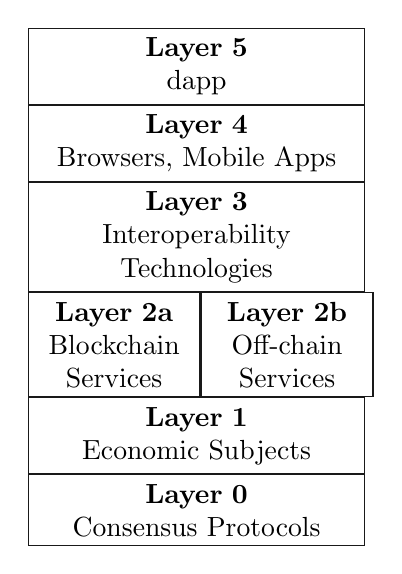
\begin{tikzpicture}
    \node (l5) [lay] {\textbf{Layer 5}\\\glspl{dapp}};
    \path (l5.south west) node [lay] (l4) {\textbf{Layer 4}\\Browsers, Mobile Apps};
    \path (l4.south west) node [lay] (l3) {\textbf{Layer 3}\\Interoperability Technologies};
    \path (l3.south west) node [mlay, anchor=north west] (l2a) {\textbf{Layer 2a}\\Blockchain Services};
    \path (l2a.east) node [mlay, anchor=west] (l2b) {\textbf{Layer 2b}\\Off-chain Services};
    \path (l2a.south west) node [lay] (l1) {\textbf{Layer 1}\\Economic Subjects};
    \path (l1.south west) node [lay] (l0) {\textbf{Layer 0}\\Consensus Protocols};
\end{tikzpicture}
    % \legend{}
    \source{Adapted from~\citeonline{vitalik2014}.}
\end{figure}

\section{Distributed applications on the electricity sector}
\label{sec:dapp}

The unique characteristic of the blockchain technology architecture by privacy levels has been allowing the development of several new applications accordingly with specific needs.
For some purposes, its use can be interpreted merely as a cloud computing service improvement,
and the \glspl{dapp} has the capability to provide a better use -- and a rapid experimentation -- of the system with full abstraction of its behavioural integration on the blockchain network~\cite{singh2017}.

It is the innovative approach of \gls{dlt} that enables diversified experimentation models,
such as the case with \gls{gd}, mainly with decentralized solar energy networks~\cite{its3}.
However, the technology configuration range capability also allows the blockchain to be used throughout the whole energy sector chain, as synthesizes the \autoref{tab:block-on-energy}.

\begin{table}[h!tbp]{\textwidth}
    \centering
    \caption{Blockchain applications on the electricity sector chain.}
    \label{tab:block-on-energy}
    % \frame{\includegraphics[clip, trim=3cm 8cm 3.25cm 13.25cm, width=\textwidth]{pics/block-on-chain.pdf}}
    \frame{\tiny
\def \bugray {\textcolor{gray}{\bullet}}
\begin{tabular}{m{2.8cm} c|c|c|c|c|c|c}
     & \multicolumn{1}{l}{\textbf{Generation}} & \multicolumn{1}{l}{\textbf{Transmission}} & \multicolumn{1}{l}{\textbf{Distribution}} & \multicolumn{1}{l}{\textbf{Trading}} & \multicolumn{1}{l}{\textbf{Sales}} & \multicolumn{1}{l}{\textbf{Metering}} & \multicolumn{1}{l}{\textbf{Other areas}} \\
 
    \multicolumn{8}{l}{\cellcolor{lightgray}B2C energy trading / peer-to-peer systems} \\
    Microgrids (peer-to-peer) & $\bugray$ & $\bugray$ & $\bugray$ \ref{brook} \textit{our proposal} & & $\bugray$ & $\bugray$ & \\
    Grid management systems & $\bugray$ & $\bugray$ & $\bugray$ & & & $\bugray$ & \ref{wien} \\
    Trading based on BC/Smart Contracts & & & \ref{pwr} & $\bugray$ \ref{alliander} \ref{ideo2} & & & \ref{wien} \\
    
    \multicolumn{8}{l}{\cellcolor{lightgray}Mobility} \\
    Charging process mgmt./payment & & & & & & & $\bugray$ \ref{rwe} \\
    Charging station handling & & & & & & & $\bugray$ \ref{rwe} \\
    Ride sharing & & & & & & & $\bugray$ \\
    
    \multicolumn{8}{l}{\cellcolor{lightgray}Asset management} \\
    Data collection/integration for individual assets ("provenance") & $\bugray$ \ref{solarcoin} & & & & & & \\
    
    \multicolumn{8}{l}{\cellcolor{lightgray}Other energy use cases} \\
    Certificate handling (e.g. for renewable energy usage) & & & & $\bugray$ & $\bugray$ & \ref{ideo1} & \ref{solshare} \\
    Payment of invoices with crypto-currencies & & & \ref{bitcoin} & $\bugray$ & $\bugray$ & & \ref{solshare} \\
    Blockchain-based supplier switching management & & & $\bugray$ & & $\bugray$ & $\bugray$ \ref{nanogrid} & \ref{ideo3} \\
\end{tabular}}
    \legend{$\bullet$ where blockchain projects are being developed.\\ $(n)$ where $n$ represents the example number presented below.}
    \source{Adapted from \citeonline{wec2017}.}
\end{table}

The electricity network use to have a top-down business model with utilities and big power generators sending electricity to customers.
Directly trade of electricity between generators and residential consumers is already a reality in the European Union (EU)~\cite{blocktrading,Brasil-futuroEE},
whilst in Brazil its mechanism is limited by the level of power consumption, and not by consumer class.

In this context,
new technologies to provide the exchange of information and to allow interactions between different autonomous agents, % agentes? conflito de nomenclatura com agentes do setor elétrico REVER!!!
embedded with artificial intelligence tools and mechanisms such as blockchain, should be a feasible solution and a trend for the next few years~\cite{Coelho2017MAS}. %[ Coelho et al., 2017].
% The presence of prosumers into the electricity market sustained by blockchain allows the share and update of data by multiple unknown parties in a trusty and verified manner~\cite{peck2017,wec2017}.
As a result, the blockchain projects can overcome the challenges with decentralized energy systems optimization,
leaving new approaches to arise, such as real-time pricing, consumers awareness about personal power consumption, prosumers awareness about when their generation is most needed, and social awareness about its impact on the grid~\cite{peck2017,wec2017}.

From this premise, worldwide solutions are being developed to enable the active participation of consumers in the electricity market as shown on \autoref{tab:block-on-energy} and described on the following \autoref{ssec:propostas}.
Therefore, for the Brazilian case, prosumers could leave a position of just accumulate energy credits to an active position, in which the excess power generated could be converted into profit. % clearing = compensação!!!

\subsection{New electricity market examples}% accordingly with \autoref{tab:block-on-energy}}
\label{ssec:propostas}

% More valuable examples (29/06/19):
% - https://innovationatwork.ieee.org/honda-gm-research-electric-vehicles-smart-grid-blockchain/
% - https://innovationatwork.ieee.org/4-blockchain-energy-companies-to-watch-in-2019/

\begin{enumerate}[label={\textcolor{gray}{(\arabic*)}}, font={\small\bfseries}]

    \item\label{solarcoin} In a more simple and international way, the \emph{SolarCoin} is a digital asset that rewards owners of solar power generation, being basically a technology to encourage decentralized, clean, and renewable energy generation,
    which aims to reduce the payback time for the solar installations~\cite{mit-dci}.
    Its crypto-currency \emph{solarcoin (SLR)} works similarly to credit cards miles program, 1 MWh is equivalent to 1 SLR.
    
    \item\label{bitcoin} On the other hand, the Marubeni company is allowing Bitcoin payments options for electricity consumption in some regions of Japan~\cite{groarke2016}.
    While a real case application in South Africa developed by Grid Singularity%
    \footnote{\href{http://gridsingularity.com}{http://gridsingularity.com}}
    uses Bitcoin transfer for accounting clearing of electricity pre-paid system \cite{video:grid}.
    
    \item\label{solshare} In Dhaka, Bangladesh, the \emph{ME SOLshare Ltd} is a social enterprise that offers \gls{p2p} trade system for solar power generation, and finance photovoltaic installations for low-income families.
    Founded in 2014, the SOLshare operates off-grid electricity in rural areas and allows its users to earn an income directly from the energy of the Sun.
    Its goal is to empower people to become entrepreneurs, enabling the creation of a bottom up smart grid, and being ready for the future integration to the power network of the country\footnote{\href{https://www.me-solshare.com/}{https://www.me-solshare.com}}.
    
    \item\label{alliander} In a similar approach, the Alliander utility aims for ``real-time'' energy trade on the Island of Texel (Holland) with smart meters linked to blockchain technology. A new business arise towards the wholesale market~\cite{groarke2016}.
    
    \item\label{nanogrid} A case of nanogrid optimization was conducted by \citeonline{magnasco2016}, in which data from a pilot nanogrid in Bangladesh was used. The authors developed a system that uses Operations Research techniques for finding the best topology of the network, defined on real-time operation with smart switches and meters.

    \item\label{brook} In the case of the \emph{Brooklyn Microgrid}, it is still limited to some consumers in Brooklyn, New York.
    The owner of a PV power can sell its generation to a neighbor using a smart contract available by the startup LO3~\cite{blocktrading}. % [Merz , 2016]
    But this model still faces regulatory issues of energy transaction, since it is under the concession area of different distribution utilities~\cite{mangelkamp2017}, which can not occur either in Brazil as stated by national \gls{gd} legislation.

    \item\label{pwr} In Australia, \emph{Power Ledger} goes a little further into the \gls{p2p} interaction, allowing the transaction between the units of a building with other consumers of the distribution grid, thanks to its tight relationship with local utility.
    Owners of a \gls{gd} can decide for who they want to sell their surplus energy and at what price.
    In the platform provided there is a mechanism of negotiation and clearing that is transparent, auditable and automated in the benefit of prosumers and consumers~\cite{pwrledger}.
    They have already expanded to Auckland area, New Zealand, with expectations that schools, community groups and residential houses participate actively in the initiative~\cite{groarke2016}.
    
    \item\label{wien} Other actions are taking place on different uses of electricity as well.
    % For instance, \emph{Fortum} enables consumers to manage theirs home consumption over internet
    % Fortum - Finland --> não achei a prov no site da empresa!
    % "Fortum aims to enable consumers to control appliances over the internet in connected homes and view blockchains as micro demand response enabler at the device level."\cite{groarke2016}
    For instance, the \emph{Wien Energie} utility uses the distributed technology to optimize and to save costs of gas trading for power generation~\cite{groarke2016}.
    Established in Austria, the system is used to guarantee the stability of the grid in case the Sun or the wind do not attend necessary demand\cite{wien-energie2016}.
    
    \item\label{rwe} And in Germany, the \emph{RWE} together with the company \emph{Slock.it}, uses the blockchain to manage electric vehicle recharge in public charging stations.
    They use an accounting unit supported by different energy suppliers in order to provide vehicle drivers a standard method of payment.
    The RWE system is based on the product \emph{BigchainDB} by Ascribe from Berlin, but it is not yet known how smart contracts are used for unlocking charging stations~\cite{blocktrading}.
    
    \item Moreover, real market applications have been tested up by the CoLab,
    an IDEO's hub for collaborative innovation, that designs human-centered projects.
    They have built three prototypes to understand blockchain potential with electricity applications.
    \begin{enumerate*}[label={\textcolor{gray}{(10.\arabic*)}}, font={\small\bfseries}]
        \item\label{ideo1} The Smart Solar
        % https://www.ideocolab.com/prototypes/smartsolar
        directly connects a solar panel to the blockchain network in order to tracks its generation, and automatically issue a personal digital Renewable Energy Certificate (REC).
        \item\label{ideo2} The Shift
        % https://www.ideocolab.com/prototypes/shift
        is a marketplace to trade energy and a self-management device to operate under power rates flexibility.
        \item\label{ideo3} And the Plug 'n' Paid
        % https://www.ideocolab.com/prototypes/plugnpaid
        is the power device manager for homes, which uses Artificial Intelligence (AI) to adjust preferences and behaviours of homeowners looking for power efficiency.
        It also manages consumption, buys power in real time, and trades power with neighboring homes accordingly with pre-charge payment.
    \end{enumerate*}
    
    % Adicionar InternetS of Energy -- DAISEE?

\end{enumerate}